%! TeX root = openfoam_presentation.tex
\usetheme[framenumber-footline]{Mumbai}



\usepackage{forest}
\usepackage{siunitx}
\usepackage{tikz}
\usetikzlibrary{arrows, arrows.meta, positioning, trees}



\def\lapfoam{\texttt{laplacianFoam}}
\def\openfoam{\texttt{OpenFOAM}}
\def\paraview{\texttt{ParaView}}
\def\parafoam{\texttt{paraFoam}}
\newcommand{\pder}[2]{\ensuremath{\frac{\partial #1}{\partial #2}}}




\begin{document}

\title{Introduction to \openfoam}
\author{Vachan Potluri}
\date{April 2023}

{
\setbeamertemplate{footline}{}
\frame{\maketitle}
}

\begin{frame}
    \begin{block}{What}
        \begin{itemize}
            \item CFD software (but without GUI)
            \item \textbf{Open} source \textbf{F}ield \textbf{O}peration \textbf{A}nd \textbf{M}anipulation
            \item Open source $\implies$ source code is given to user
        \end{itemize}
    \end{block}
\onslide<2->
    \begin{figure}
        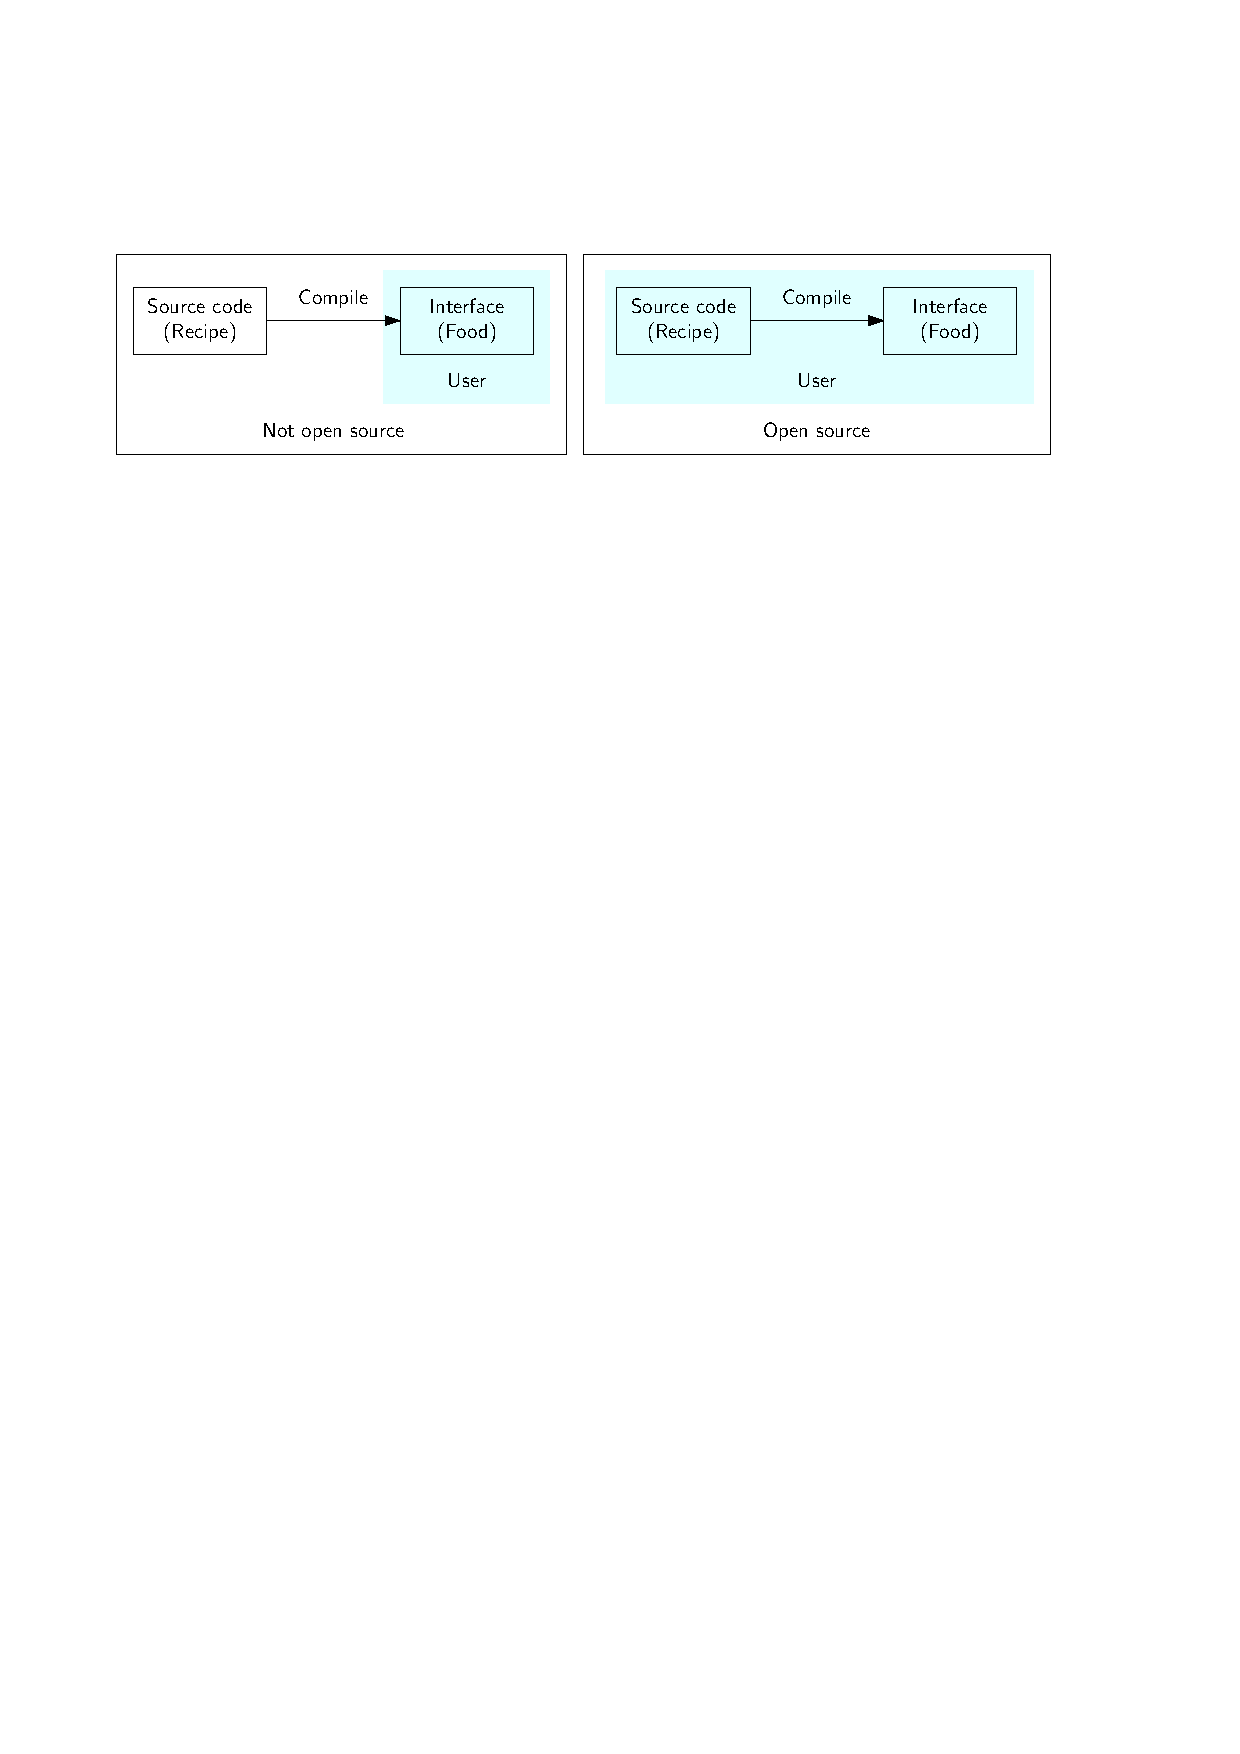
\includegraphics[width=\linewidth]{opensource_illustration}
    \end{figure}
\onslide<3->
    No GUI $\implies$ hard to learn
    \begin{block}{Why}
        \begin{itemize}
            \item Free
            \item Fast
            \item User customisable
        \end{itemize}
    \end{block}
\end{frame}

\begin{frame}{Case 1}{Heat conduction in a square plate}
    \begin{equation*}
        \pder{T}{t} = \nabla \cdot (D_T \nabla T)
    \end{equation*}
    \begin{figure}
        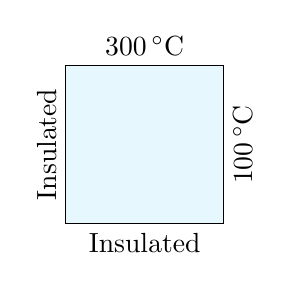
\begin{tikzpicture}[scale=2]
            \draw [fill=cyan!10] (0,0) -- node [below] {Insulated} (1,0) -- node [rotate=90, below] {\qty{100}{\degreeCelsius}} (1,1) -- node [above] {\qty{300}{\degreeCelsius}} (0,1) -- node [rotate=90, above] {Insulated} cycle;
        \end{tikzpicture}
    \end{figure}
\onslide<2->
    \begin{itemize}
        \item \lapfoam{} is the ``solver'' to be used for heat conduction equation
        \item Visualise using \parafoam
    \end{itemize}
\end{frame}

\begin{frame}{\openfoam's case setup}
    For doing \lapfoam{} simulation, create a folder with this structure
    \begin{block}{Case structure for \lapfoam}
        \begin{figure}
            \centering
            \begin{forest}
                [folder name
                    [0]
                    [constant]
                    [system]
                ]
            \end{forest}
        \end{figure}
    \end{block}
\end{frame}

\end{document}